\subsubsection{Leptonic \Vg production}
\label{sss-Vgammaprod}

%analysis CMS and ATLAS.
%	ATLAS W/Z gam, Phys. Rev. D 87, 112003 (2013), http://arxiv.org/abs/1302.1283
%       ATLAS Z gam (gam), PRD accepted (2016), http://arxiv.org/abs/1604.05232
%	CMS W/Z gam, Phys. Rev. D 89 (2014) 092005, http://arxiv.org/abs/1308.6832
%	CMS llgam (8TeV 20ifb),JHEP 04 (2015) 164, http://arxiv.org/abs/1502.05664
%	CMS vvgam 7TeV, JHEP 10 (2013) 164, http://arxiv.org/abs/1309.1117
%	CMS vvgam 8 TeV, https://cms-physics.web.cern.ch/cms-physics/public/SMP-14-019-pas.pdf (soon submitted), http://arxiv.org/abs/1602.07152  (Khachatryan:2016yro)


%intro
The di-boson system of a massive vector boson and a photon has a similar 
electroweak production rate as the massive di-boson final states. Initial
and final state QED radiation from the incoming quarks and
outgoing charged decay products are dominating the total cross section 
for this final state. To compare to theory, fiducial cross sections are defined
that enhance the electroweak component. The \Wg process has been studied in the
leptonic decay $\Wglvg$ and limits on charged ATGC are set. The \Zg process
has two leptonic decay modes \Zgllg\; and \Zgvvg, which are both sensitive
to neutral ATGC. Due to the absence of final state radiation in \Ztovv\;
and the higher branching ratio compared to \Ztoll\;
the $\vv$ final state is more sensitive to ATGC.
%BACKGROUNDS
The main background arises from \W+jets and \Z+jets production, where one 
jet is misidentified as an isolated photon. Data driven techniques are employed
to estimate this background. Other important sources of backgrounds are multi-jet production
and \ttbar\; pair production in association with a photon, and are estimated from simulation.
The achieved signal to background ratios range from about 0.8 -- 1.5 for \Wglvg\; to 3.5 -- 7 for \Ztoll\;
depending on channel and experiment. 

%RESULT SUMMARY
ATLAS and CMS have published measurements of fiducial production cross sections of
\Wglvg, \Zgllg at $\rts=7\TeV$ and $\rts=8\TeV$. 
The fiducial volume is defined at particle level with kinematic selection criteria 
on objects and at the event level. ATLAS and CMS differ in the definitions 
of the fiducial cross section, leading to differences in the predicted cross sections. 
The cross-section for \Zgllg\; and $\Wglvg$ is defined as 
$\pt(\gamma)>15\GeV$,$\Delta(\ell,\gamma)>0.7$, and additionally for \Zg\; $m(\ell\ell)>50 (40) \GeV)$ 
for CMS (ATLAS). ATLAS further requires $|\eta(\ell)|<2.47$,  $|\eta(\gamma)|<2.37$, and 
$\ET(jet) >30\GeV$, $|\eta(jet)|<4.4$, $\Delta R (jet,x) > 0.3$ for jets with $x$ being a lepton, jet, or photon. 
For the \Zgvvg\; process the cross section is defined as $\ET(\gamma)>145 (100, 130)\GeV$, 
$|\eta(\gamma)|<1.4(2.37)$, $\pt(\nu\nu)>130(90, 100)$ for CMS (ATLAS 7 TeV \cite{Chatrchyan:2013nda}, and 8 TeV \cite{Aad:2016sau}).
A summary of the measurements is given in Table~\ref{tab:sss-Vgamma-prod-xsec}. Overall the agreement
of the measured and NLO predicted exclusive cross sections is good, while the measured inclusive cross sections tend to be
higher then the NLO prediction, which may be partially attributed to corrections at NNLO in $\alpha_s$.


\begin{table}[htp]
\begin{center}
\resizebox{\textwidth}{!}{
\begin{tabular}{|c|c|c|c|c|c|c|}
Experiment & process & cross section & \rts\;[TeV] & measured  & predicted  & reference  \\ \hline
ATLAS	   & \Wglvg  & inclusive     & 7 & 2.77 $\pm$ 0.03 (stat) $\pm$ 0.33 (syst) $\pm$ 0.14 (lumi) pb         & 1.96 $\pm$ 0.17 pb  & \cite{Aad:2013izg} \\ 
ATLAS	   & \Wglvg  & exclusive     & 7  &  1.76 $\pm$ 0.03 (stat) $\pm$ 0.21 (syst) $\pm$ 0.08 (lumi) pb        & 1.39 $\pm$ 0.13 pb & \cite{Aad:2013izg} \\ 
ATLAS	   & \Zgllg  & inclusive      & 7  & 1.31 $\pm$ 0.02 (stat) $\pm$ 0.11 (syst) $\pm$ 0.05 (lumi) pb        & 1.18 $\pm$ 0.05 pb         & \cite{Aad:2013izg} \\ 
ATLAS	   & \Zgllg  & exclusive      & 7  & 1.05 $\pm$ 0.02 (stat) $\pm$ 0.10 (syst) $\pm$ 0.04 (lumi) pb       & 1.06 $\pm$ 0.05 pb          & \cite{Aad:2013izg} \\ 
ATLAS  	   & \Zgvvg  & inclusive      & 7  & 0.133 $\pm$ 0.013 (stat) $\pm$ 0.020 (syst) $\pm$ 0.005 (lumi) pb         & 0.156 $\pm$ 0.012 pb          & \cite{Chatrchyan:2013nda} \\ 
ATLAS  	   & \Zgvvg  & exclusive      & 7  &  0.116 $\pm$ 0.010 (stat) $\pm$ 0.013 (syst) $\pm$ 0.004 (lumi) pb      &  0.115 $\pm$ 0.009 pb         & \cite{Chatrchyan:2013nda} \\ 
CMS  	   & \Zgllg  & inclusive      & 7  &   5.33 $\pm$ 0.08 (stat) $\pm$ 0.25 (syst) $\pm$ 0.12 (lumi) pb       & 5.45 $\pm$ 0.27 pb           & \cite{Chatrchyan:2013fya} \\ 
CMS  	   & \Wglvg  & inclusive      & 7  &  37.0 $\pm$ 0.8 (stat) $\pm$ 4.0 (syst) $\pm$ 0.8 (lumi) pb         & 31.8 $\pm$ 1.8 pb  & \cite{Chatrchyan:2013fya} \\ 
CMS  	   & \Zgvvg  & inclusive      & 7  &  21.1 $\pm$ 4.2 (stat.) $\pm$ 4.3 (syst) $\pm$ 0.5 (lumi) fb        &  21.9 $\pm$ 1.1 fb   & \cite{Chatrchyan:2013nda} \\ 

ATLAS	   & \Zgllg  & inclusive      & 8  & 1.51 $\pm$ 0.01 (stat) $\pm$ 0.08 (syst) $\pm$ 0.03 (lumi) pb        & 1.35 $\pm$ 0.07 pb         & \cite{Aad:2016sau} \\ 
ATLAS	   & \Zgllg  & exclusive      & 8  & 1.19 $\pm$ 0.01 (stat) $\pm$ 0.07 (syst) $\pm$ 0.02 (lumi) pb       & 1.19 $\pm$ 0.08 pb          & \cite{Aad:2016sau} \\ 
ATLAS  	   & \Zgvvg  & inclusive      & 8  & 68 $\pm$ 4 (stat) $\pm$ 32 (syst) $\pm$ 1 (lumi) fb         & 68 $\pm$ 2 fb          & \cite{Aad:2016sau} \\ 
ATLAS  	   & \Zgvvg  & exclusive      & 8  & 43 $\pm$ 2 (stat) $\pm$ 10 (syst) $\pm$ 1 (lumi) fb      &  51 $\pm$ 2 fb         & \cite{Aad:2016sau} \\ 
CMS  	   & \Zgllg  & inclusive      & 8  &  2063 $\pm$ 19 (stat) $\pm$ 98 (syst) $\pm$ 54 (lumi) fb  &  2100 $\pm$ 120 fb          & \cite{Khachatryan:2015kea} \\ 
CMS  	   & \Zgllg  & exclusive      & 8  &     1770 $\pm$ 18 (stat) $\pm$ 115 (syst) $\pm$ 46 (lumi) fb     &  1800 $\pm$ 120 fb          & \cite{Khachatryan:2015kea} \\ 
CMS  	   & \Zgvvg  & inclusive      & 8  &     52.7 $\pm$ 2.1 (stat) $\pm$ 6.4 (syst) $\pm$ 1.4 (lumi) fb     & 40.7 $\pm$ 4.9 fb       & \cite{Khachatryan:2016yro} \\ 
\end{tabular}
}
\caption{Summary of measured \Vg production cross sections from ATLAS and CMS
at 7 and 8 TeV center-of-mass energies in the \Wglvg, \Zgvvg\; and \Zgllg\; final states. The inclusive cross section is for $n_{jet} \geq 0$ and the exclusive cross section is for $n_{jet}=0$. The
cross section definitions differ for ATLAS and CMS and the numerical values are not directly 
comparable. For the \Zgvvg process ATLAS uses a different cross section definition between the 7 TeV and 8 TeV measurements.}
\end{center}
\label{tab:sss-Vgamma-prod-xsec}
\end{table}

To extract limits on ATGC parameters the transverse momentum of the photon $\pt(\gamma)$ is used 
by CMS, while ATLAS uses a more conservative approach by combining the observed 
number of exclusive \Vg candidate events with $\ET(\gamma)>100\GeV$.  
The channel most sensitive to the neutral TGC couplings \hthreev, \hfourv\; as defined 
in~\cite{PhysRevD.47.4889} is \Zgvvg\;
due to the high branching ratio of $\Zzero$ to neutrinos of 20\%. 
Figure~\ref{fig:sss-inclboson-diboson-Vgamma-zgamvvgamptgam} shows the transverse momentum of the photon at 8~\TeV\; measured by CMS in the \Zgvvg\; channel~\cite{Khachatryan:2016yro} together with a hypothetical
TGC signal.

%FIGURE Zgam pt(gam)
% 
% http://cms-results.web.cern.ch/cms-results/public-results/publications/SMP-14-019/index.html
% http://cms-results.web.cern.ch/cms-results/public-results/publications/SMP-14-019/CMS-SMP-14-019_Figure_002-a.png
% CMS Zgam vvgam 8 TeV
\begin{figure}[htbp]
  \begin{center}
  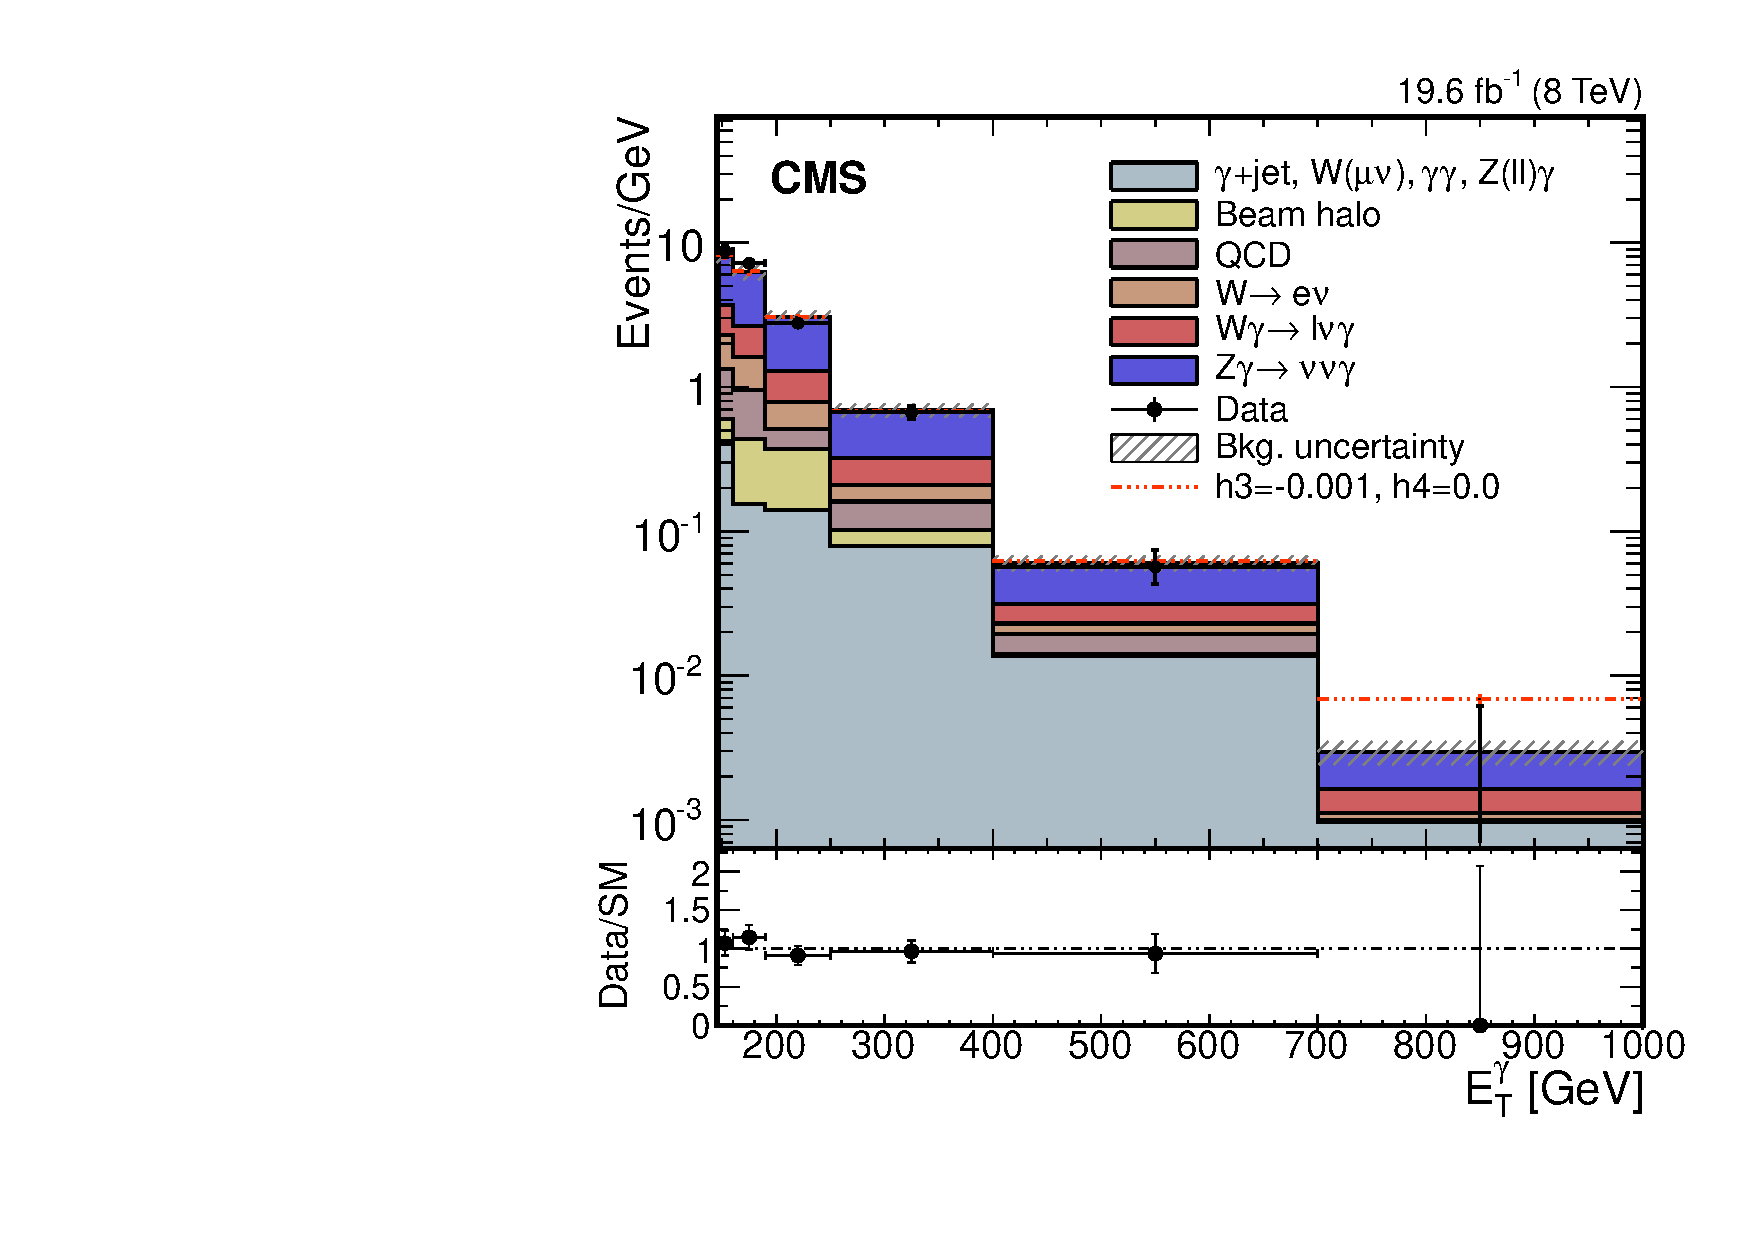
\includegraphics[width=0.45\textwidth]{figures/sss-inclboson-diboson-Vgamma-zgamvvgamptgam.pdf}
  \caption{ 
  The $\ET(\gamma)$ distribution from CMS~\cite{Khachatryan:2016yro} in data (points) compared to signal and estimated background contributions (histogram). A ATGC signal with $\hthreev=-0.001$ is 
  shown (dot-dashed histogram) for comparison. The background uncertainty includes statistical and systematic contributions. 
}
\label{fig:sss-inclboson-diboson-Vgamma-zgamvvgamptgam}
\end{center}
\end{figure}

The resulting 95\% CL limits for charged (\Wg) and neutral (\Zg) TGC are listed in Table~\ref{tab:sss-Vgamma-ATGC}. For comparison, only limits obtained without the use of a form factor are listed. ATLAS
also provides limits with unitarity-preserving form factors, and in case of the $\rts=8\TeV$  analysis limits as a function of the dipole form factor scale $\Lambda$~\cite{Aad:2016sau}. 

\begin{table}\centering
\resizebox{\textwidth}{!}{
\begin{tabular}{|c|c|c|c|c|c|c|c|}
& & & & \multicolumn{2}{c} {ATLAS} & CMS   \\ 
& Process & \rts\;[TeV] & $\mathcal{L} [\ifb]$ ATLAS, CMS & Observed & Expected & Observed  \\
\hline

$\dkg$&\Wglvg& 7 &$4.6,5$& $[-0.41, 0.46]$ & $[-0.38, 0.43]$ & $[-0.38, 0.29]$  \\
$\lg$&\Wglvg& 7 &$4.6,5$& $[-0.065, 0.061]$ & $[-0.060, 0.056]$ & $[-0.050, 0.037]$ \\
$\hthreeg$ &\Zgllg,\Zgvvg& 7 &$4.6,5.0$& $[-0.015, 0.016]$ & $[-0.017, 0.018]$ & $<2.9\cdot 10^{-3}$ \\
$\hthreez$ &\Zgllg,\Zgvvg& 7 &$4.6,5.0$& $[-0.013, 0.014]$ & $[-0.015, 0.016]$ & $<2.7 \cdot 10^{-3}$  \\
$\hfourg$ & \Zgllg,\Zgvvg & 7 &$4.6,5.0$& $[-9.4 \cdot 10^{-5}, 9.2 \cdot 10^{-5}]$ & $[-1.0 \cdot 10^{-4}, 1.0 \cdot 10^{4}]$ & $<1.5 \cdot 10^{-5}$  \\
$\hfourz$ & \Zgllg,\Zgvvg & 7 &$4.6,5.0$& $[-8.7 \cdot 10^{-5}, 8.7 \cdot 10^{-5}]$ & $[-9.7 \cdot 10^{-5}, 9.7 \cdot 10^{5}]$ & $<1.3 \cdot 10^{-5}$  \\
$\hthreeg$ &\Zgllg,\Zgvvg& 8 &$20.3, - $& $[-9.5\cdot 10^{-4}, 9.9\cdot 10^{-4}]$ & $[-1.8\cdot 10^{-3}, 1.8\cdot 10^{-3}]$ & -- \\
$\hthreez$ &\Zgllg,\Zgvvg& 8 &$20.3, - $& $[-7.8\cdot 10^{-4}, 8.6\cdot 10^{-4}]$ & $[-1.5\cdot 10^{-3}, 1.5\cdot 10^{-3}]$ & -- \\
$\hfourg$  &\Zgllg,\Zgvvg& 8 &$20.3, - $& $[-3.2\cdot 10^{-6}, 3.2\cdot 10^{-6}]$ & $[-6.0\cdot 10^{-6}, 5.9\cdot 10^{-6}]$ & -- \\
$\hfourz$  &\Zgllg,\Zgvvg& 8 &$20.3, - $& $[-3.0\cdot 10^{-6}, 2.9\cdot 10^{-6}]$ & $[-5.5\cdot 10^{-6}, 5.4\cdot 10^{-6}]$ & -- \\
$\hthreeg$ &\Zgllg& 8 &$-, 19.5$& -- & -- & $[-4.6 \cdot 10^{-3}, 4.6 \cdot 10^{-3}]$ \\
$\hthreez$ &\Zgllg& 8 &$-, 19.5$& -- & -- & $[-3.8 \cdot 10^{-3}, 3.7 \cdot 10^{-3}]$ \\
$\hfourg$ &\Zgllg& 8 &$-, 19.5$& -- & -- & $[-3.6 \cdot 10^{-5}, 3.5 \cdot 10^{-5}]$ \\
$\hfourz$ &\Zgllg& 8 &$-, 19.5$& -- & -- & $[-3.1 \cdot 10^{-5}, 3.0 \cdot 10^{-5}]$ \\
$\hthreeg$ &\Zgvvg& 8 &$-, 19.5$& -- & -- & $[-1.1 \cdot 10^{-3}, 0.9 \cdot 10^{-3}]$ \\
$\hthreez$ &\Zgvvg& 8 &$-, 19.5$& -- & -- & $[-1.5 \cdot 10^{-3}, 1.6 \cdot 10^{-3}]$ \\
$\hfourg$ &\Zgvvg& 8 &$-, 19.5$& -- & -- & $[-3.8 \cdot 10^{-6}, 4.3 \cdot 10^{-6}]$ \\
$\hfourz$ &\Zgvvg& 8 &$-, 19.5$& -- & -- & $[-3.9 \cdot 10^{-6}, 4.5 \cdot 10^{-6}]$ \\

\end{tabular}
}
\caption{Expected and observed 95\% CL on \hthreeg, \hthreez, \hfourg, and \hfourz\; measured in the 
\Zgllg\; and \Zgvvg\; final states from the ATLAS and CMS collaborations.}
\label{tab:sss-Vgamma-ATGC}
\end{table}





